% Options for packages loaded elsewhere
\PassOptionsToPackage{unicode}{hyperref}
\PassOptionsToPackage{hyphens}{url}
%
\documentclass[
]{book}
\usepackage{lmodern}
\usepackage{amssymb,amsmath}
\usepackage{ifxetex,ifluatex}
\ifnum 0\ifxetex 1\fi\ifluatex 1\fi=0 % if pdftex
  \usepackage[T1]{fontenc}
  \usepackage[utf8]{inputenc}
  \usepackage{textcomp} % provide euro and other symbols
\else % if luatex or xetex
  \usepackage{unicode-math}
  \defaultfontfeatures{Scale=MatchLowercase}
  \defaultfontfeatures[\rmfamily]{Ligatures=TeX,Scale=1}
\fi
% Use upquote if available, for straight quotes in verbatim environments
\IfFileExists{upquote.sty}{\usepackage{upquote}}{}
\IfFileExists{microtype.sty}{% use microtype if available
  \usepackage[]{microtype}
  \UseMicrotypeSet[protrusion]{basicmath} % disable protrusion for tt fonts
}{}
\makeatletter
\@ifundefined{KOMAClassName}{% if non-KOMA class
  \IfFileExists{parskip.sty}{%
    \usepackage{parskip}
  }{% else
    \setlength{\parindent}{0pt}
    \setlength{\parskip}{6pt plus 2pt minus 1pt}}
}{% if KOMA class
  \KOMAoptions{parskip=half}}
\makeatother
\usepackage{xcolor}
\IfFileExists{xurl.sty}{\usepackage{xurl}}{} % add URL line breaks if available
\IfFileExists{bookmark.sty}{\usepackage{bookmark}}{\usepackage{hyperref}}
\hypersetup{
  pdftitle={CH3/40227 Advanced Spectroscopic Techniques},
  pdfauthor={Fiona Dickinson},
  hidelinks,
  pdfcreator={LaTeX via pandoc}}
\urlstyle{same} % disable monospaced font for URLs
\usepackage{longtable,booktabs}
% Correct order of tables after \paragraph or \subparagraph
\usepackage{etoolbox}
\makeatletter
\patchcmd\longtable{\par}{\if@noskipsec\mbox{}\fi\par}{}{}
\makeatother
% Allow footnotes in longtable head/foot
\IfFileExists{footnotehyper.sty}{\usepackage{footnotehyper}}{\usepackage{footnote}}
\makesavenoteenv{longtable}
\usepackage{graphicx,grffile}
\makeatletter
\def\maxwidth{\ifdim\Gin@nat@width>\linewidth\linewidth\else\Gin@nat@width\fi}
\def\maxheight{\ifdim\Gin@nat@height>\textheight\textheight\else\Gin@nat@height\fi}
\makeatother
% Scale images if necessary, so that they will not overflow the page
% margins by default, and it is still possible to overwrite the defaults
% using explicit options in \includegraphics[width, height, ...]{}
\setkeys{Gin}{width=\maxwidth,height=\maxheight,keepaspectratio}
% Set default figure placement to htbp
\makeatletter
\def\fps@figure{htbp}
\makeatother
\setlength{\emergencystretch}{3em} % prevent overfull lines
\providecommand{\tightlist}{%
  \setlength{\itemsep}{0pt}\setlength{\parskip}{0pt}}
\setcounter{secnumdepth}{5}
\usepackage{booktabs}
\usepackage{amsthm}
\makeatletter
\def\thm@space@setup{%
  \thm@preskip=8pt plus 2pt minus 4pt
  \thm@postskip=\thm@preskip
}
\makeatother
\usepackage[]{natbib}
\bibliographystyle{apalike}

\title{CH3/40227 Advanced Spectroscopic Techniques}
\author{Fiona Dickinson}
\date{2021-02-16}

\begin{document}
\maketitle

{
\setcounter{tocdepth}{1}
\tableofcontents
}
\hypertarget{ch340227-advanced-spectroscopic-techniques}{%
\chapter*{CH3/40227 Advanced Spectroscopic Techniques}\label{ch340227-advanced-spectroscopic-techniques}}
\addcontentsline{toc}{chapter}{CH3/40227 Advanced Spectroscopic Techniques}

\hypertarget{welcome-preliminary-infomation}{%
\section*{Welcome \& Preliminary Infomation}\label{welcome-preliminary-infomation}}
\addcontentsline{toc}{section}{Welcome \& Preliminary Infomation}

Welcome to the coursepage for CH30227 \& CH40227 Advanced Spectroscopic Techniques. The notes have been prepared in a package called BookDown for RStudio so that the equations are accessible to screen readers. However, by providing the notes as a .html webpage I can also embed short videos to further describe some of the topics. Further you can download the material in a format that suits you (either pdf or epub) to view offline, or change the way this document appears for ease of reading.

The course is entirely taught by Dr Fiona Dickinson.

\hypertarget{prerequisite-knowledge}{%
\subsection*{Prerequisite knowledge}\label{prerequisite-knowledge}}
\addcontentsline{toc}{subsection}{Prerequisite knowledge}

The course relies extensively on concepts from CH30129 (or CH30217) Photochemistry as well as material from the spectroscopy section of CH10137/8, and the quantum mechanics of CH20151/2. However more generic skills, such as experiment planning, and drawing conclusions on data will form an important strand to this course.

\hypertarget{assessment-for-this-course}{%
\subsection*{Assessment for this course}\label{assessment-for-this-course}}
\addcontentsline{toc}{subsection}{Assessment for this course}

The course is assessed by a `1 hour' exam, this is to say it should take an hour to complete, exam details will be shared centrally later in the semester.

The exam format will contain 2 x 25 mark questions. The questions will likely contain two or more of the following: data to examine, description of a spectrometer or spectrometer component, and design of experiments.

\hypertarget{feedback-for-this-course}{%
\subsection*{Feedback for this course}\label{feedback-for-this-course}}
\addcontentsline{toc}{subsection}{Feedback for this course}

Much of the work will be peer based in small groups, and you will provide feedback to each other. In wrapping up these discussions I will also provide feedback to discussions.

I appreciate your understanding that feedback may be delayed during these uncertain times as I have childcare responsibilities.

I will not provide model answers for past exam questions, this is because there will be multiple ways in which marks may be achieved. Instead I will happily provide feedback on your attempts at past papers. All I ask is:

\begin{itemize}
\tightlist
\item
  papers are received in good time
\item
  when you attempt papers you try and replicate the exam conditions (i.e.~do it alone, in one sitting in a limited period)
\item
  you do not submit more than one past paper at a time (I am happy to go through more than one feedback cycle, but want you to reflect on the feedback you have received)
\item
  you highlight sections where you particularly want feedback
\item
  you provide the file as a .pdf, with the file name containing your username, the year of paper attempted and the unit code
\item
  please space out work enough so that I can write feedback
\end{itemize}

\hypertarget{week-1-tasks}{%
\section*{Week 1 tasks}\label{week-1-tasks}}
\addcontentsline{toc}{section}{Week 1 tasks}

I set a number of week 1 tasks.

\begin{itemize}
\item
  For the `spectrometer components document' on Teams, please divide the work between you, and write a few sentences (and include figures if relevant) for your chosen component(s). This is a shared document and is hosted on Teams because I can't work out how to do it on Moodle\ldots{} (the CH40227 class will act as editors to this body or work).
\item
  Think about the spectroscopic techniques you have used previously (you should all have used at least one of UV/vis, IR and fluorescence), think about what components may have been in the `beige box' and how these differ between different spectrometers\ldots{}
\item
  Remember to let me know if you want particular groups in the zoom chat (CH30227 only)
\end{itemize}

\hypertarget{report-errors}{%
\section*{Report errors}\label{report-errors}}
\addcontentsline{toc}{section}{Report errors}

If you spot any errors, please message me in Teams or (if this works), report on the error log below

Loading\ldots{}

\hypertarget{edit-log}{%
\section*{Edit log}\label{edit-log}}
\addcontentsline{toc}{section}{Edit log}

Chapters 1 \& 2 130221
Initial commit 010221

\hypertarget{ch:UVvisfluorIR}{%
\chapter{Basic Spectroscopies}\label{ch:UVvisfluorIR}}

Please scroll to the bottom to find a summary video on UV/vis and fluroescence spectroscopy.

\hypertarget{sec:UV}{%
\section{UV/Vis}\label{sec:UV}}

\hypertarget{the-beer-lambert-law}{%
\subsection{The Beer-Lambert Law}\label{the-beer-lambert-law}}

The intensity of incident light (\(I_0\)) passing through a sample falls exponentially, this is described by the Beer-Lambert Law. The empirical equation (equation \eqref{eq:BeerLambert}, figure \ref{fig:BeerLambert}) implies that the probability of a photon being absorbed at any point is the same (much like first order kinetics), and the amount of the total absorption depends upon the the concentration of the sample, c, and the `path length', l.

The amount of absorbance, A, is dependent upon the wavelength of the incident light, and the constant of proportionality, \(\varepsilon\) (here called the molar extinction coefficient), is consequently also wavelength dependent.

\begin{equation}
\log \frac{I_0}{I}=A=\varepsilon cl
\label{eq:BeerLambert}
\end{equation}

The wavelength of a particular value of the molar exctinction coefficient is often represted as a subscript, \(\varepsilon _\lambda\)

\begin{figure}

{\centering 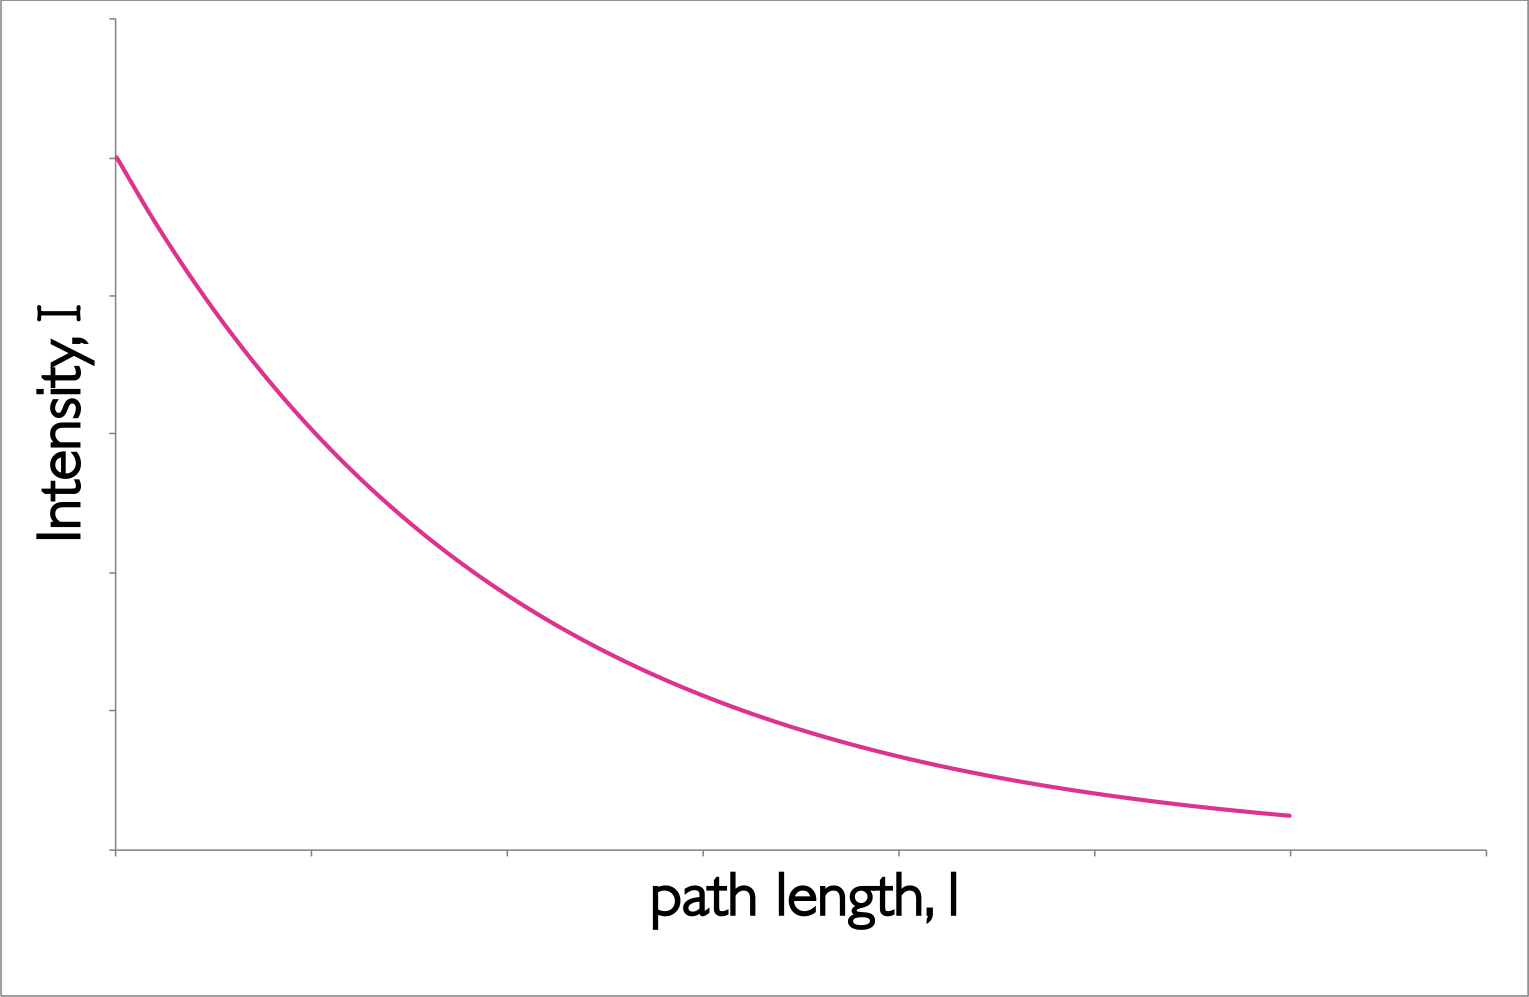
\includegraphics[width=0.5\linewidth]{images/BeerLambert} 

}

\caption{The decay of intensity of monochromatic incident light through a uniformly absorbing medium. The decay follows an exponential pattern as elucidated in the Beer-Lambert equation.}\label{fig:BeerLambert}
\end{figure}

The Beer-Lambert law makes a number of assumptions, and this exponential decay of the intensity of light is an important factor.When using the Beer-Lambert law you consider the intensity of the incident radiation, there is an assumption that the intensity of the radiation reaching each part of the sample does not deviate much from this. Hence high absorbing samples tend to show strong deviation from the Beer-Lambert's linear relationship.

The Beer-Lambert law also has to make a number of other `reasonable' considerations:

\begin{itemize}
\tightlist
\item
  The solutions is well mixed, and absorbers are homogeneously distributed in solution.
\item
  The absorbers do not scatter radiation (all particles will Rayleigh and Raman scatter but this is normally considerably less intense than absorption). Consequently solutions should be optically transparent as optically opaque solutions (such as colloidal solutions) have considerably stronger scattering.
\item
  The absorbers acts independently of each other, this means solutions need to be at a reasonably low concentration (typically less than 0.01 M, or maybe even less depending on the species) so as to avoid electrostatic or \(\pi\) stacking interactions between the chromophores.This is in part important because light is only absorbed when the polarisation of the light is aligned with the transition dipole moment.
\item
  The incident radiation is collimated, and each photon should pass through the same path length.
\item
  The sample holder (cuvette) is optically `pure' such that reflections are avoided (linked to the assumption above).
\item
  The incident radiation is monochromatic, or at the very least has a band width more narrow than the band width of the absorbing transition (this is usually not an issue for molecular systems as bandwidths are usually 10s or more of nm wide, but for atomic or ion spectroscopy where bandwidths are \textless0.02 nm this is a factor which must be carefully considered.
\item
  The incident radiation does not noticeably affect the concentration of the ground state, in other words the amount of excited states generated must be kept small as when we are talking about the absorption of a chromophore the concentration of that chromophore that appears in the Beer-Lambert equation is the ground state concentration.
\item
  There is no measurable emission from the sample.
\end{itemize}

\hypertarget{sec:usingUV}{%
\subsection{Using UV/Vis}\label{sec:usingUV}}

These assumptions become important as we start to consider more complicated techniques than the most basic absorption spectrometery, however to ensure we are following these limits on the Beer-Lambert law it is rare for spectroscopists to work with sample absorbances above 0.1 (the point where \textasciitilde20 \% of the light is absorbed).

To do this either the path length (\(l\)) is reduced or the concentration (\(c\)) of the sample is reduced.

UV/vis is simplest to use on solution based systems as one of the assumptions of the Beer-Lambert law is that the transition dipole moments are randomly aligned. The use of non-randomly aligned transition dipole moments is the basis of the technique linear dichroism (LD) \ref{sec:LD}.

\hypertarget{sec:UVinstrument}{%
\subsection{The UV/Vis instrument}\label{sec:UVinstrument}}

\begin{figure}

{\centering 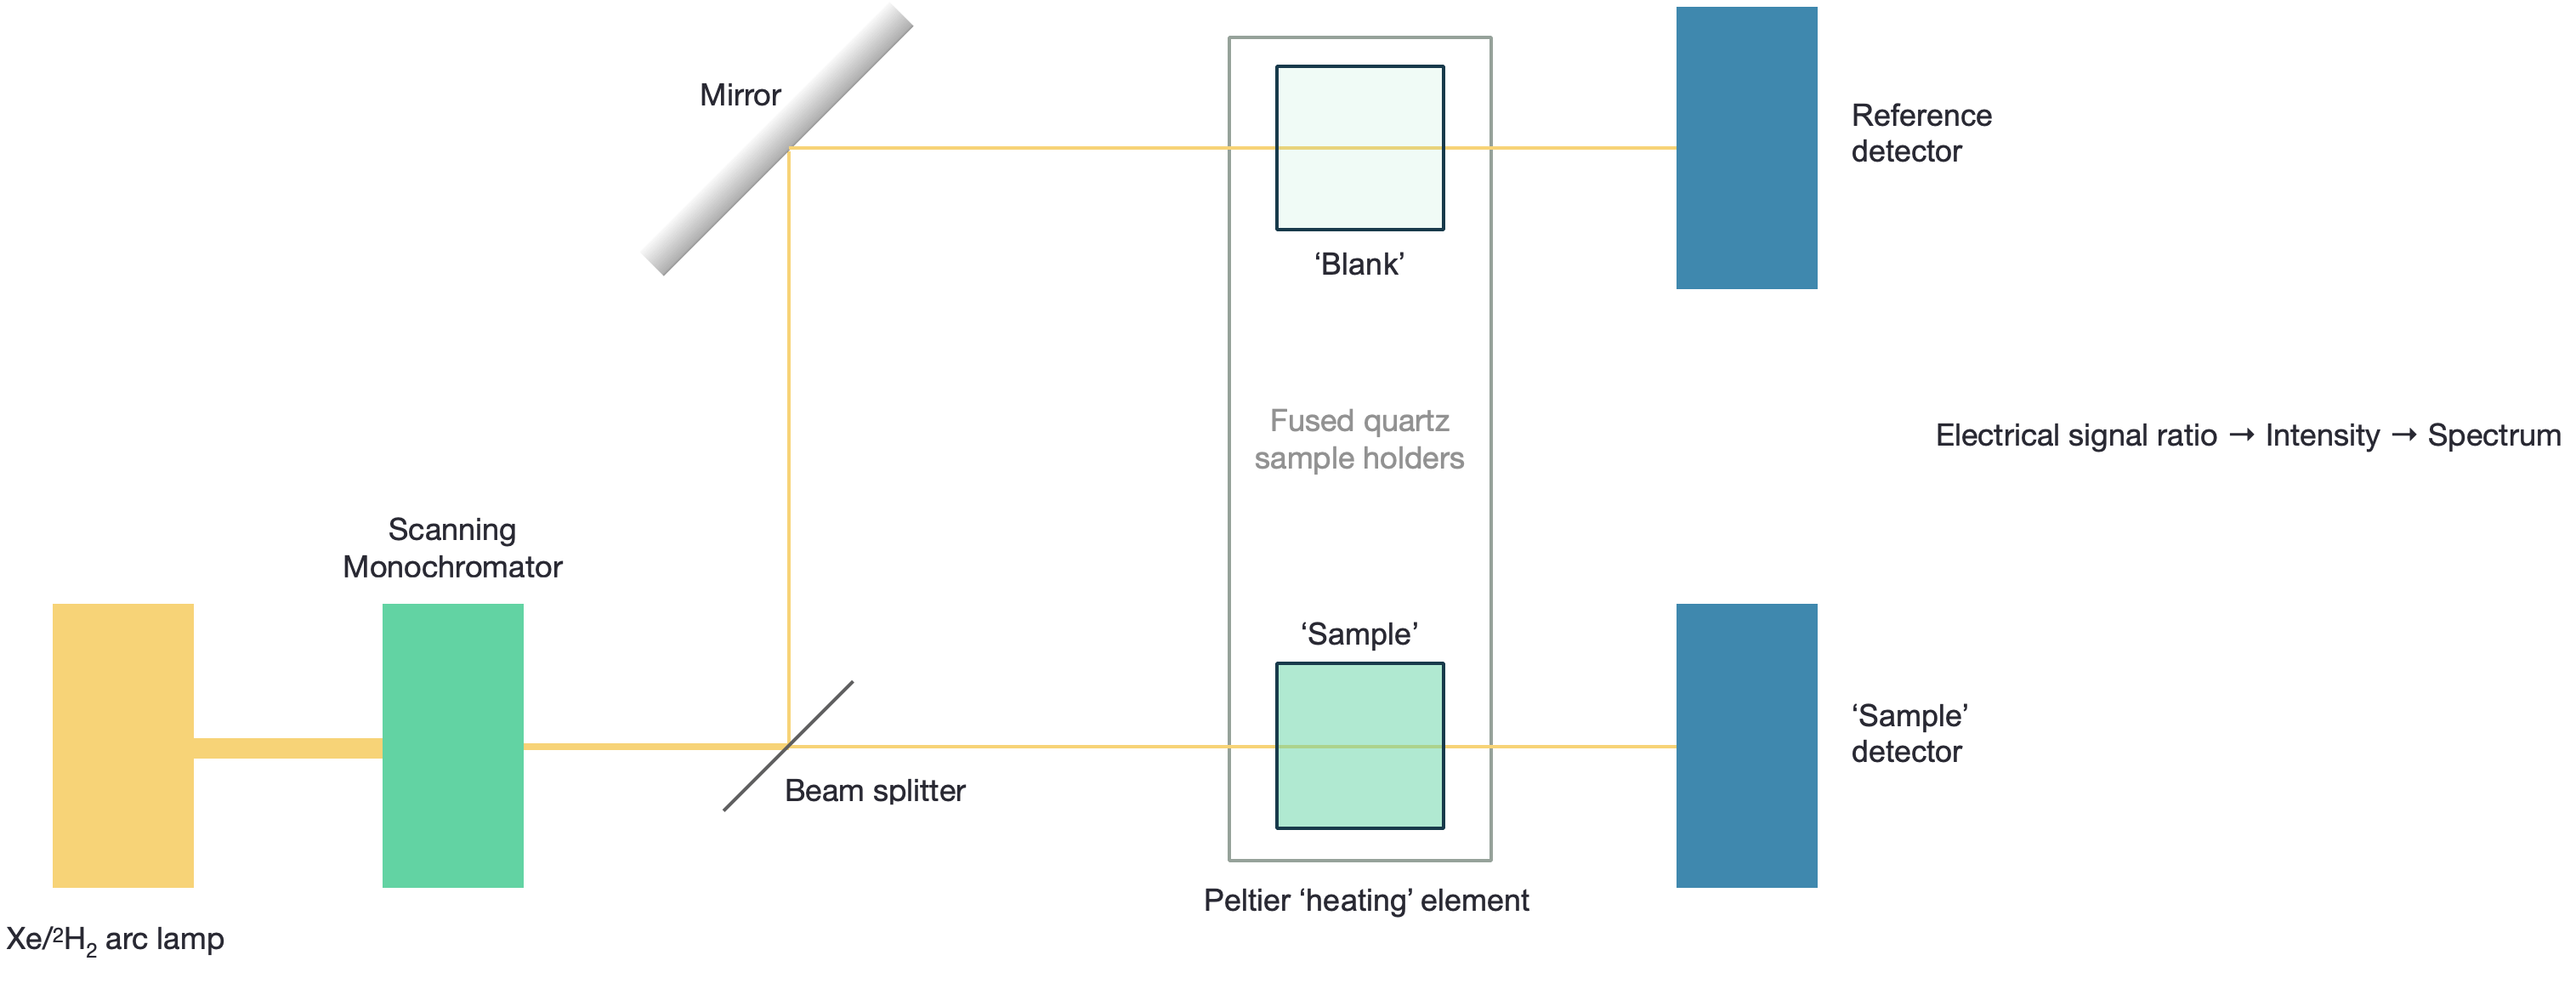
\includegraphics[width=1\linewidth]{images/UVvis} 

}

\caption{The UV/Visible spectrophotometer consists of a source of light, wavelength selector, cell holder and detector, however the complexity of each of these is very much dependent upon the instrument used.}\label{fig:UV}
\end{figure}

Figure \ref{fig:UV} shows the schematic of a `dual beam' UV/Vis spectrophotometer, this would be a higher end instrument.

The most basic versions (and the version you may have used in the lab) are single beam instruments, whereby \(I_0\) is determined indirectly. Some instruments use a `blank path' which does not allow for a `blank' reference cuvette, to allow light to reach the detector, in this case it is a single detector for both paths, with the beam of light beign selected by use of a rotaing chopper. Historically photodiodes were used as the detectors, however the use of `echelle' (2-dimensional) diffraction gratings have increasingly meant that CCDs may be used for optaining the whole spectrum instantly.

The use of a heating block for the sample means that a range of interesting studies may occur from the melting of DNA and proteins (see CH30129/CH30217 notes on hypochromicity), and the temperature dependent release of drug molecules. However, this feature again is only on higher end instruments.

\hypertarget{sec:fluorimeter}{%
\section{Fluorimeters}\label{sec:fluorimeter}}

\begin{figure}

{\centering 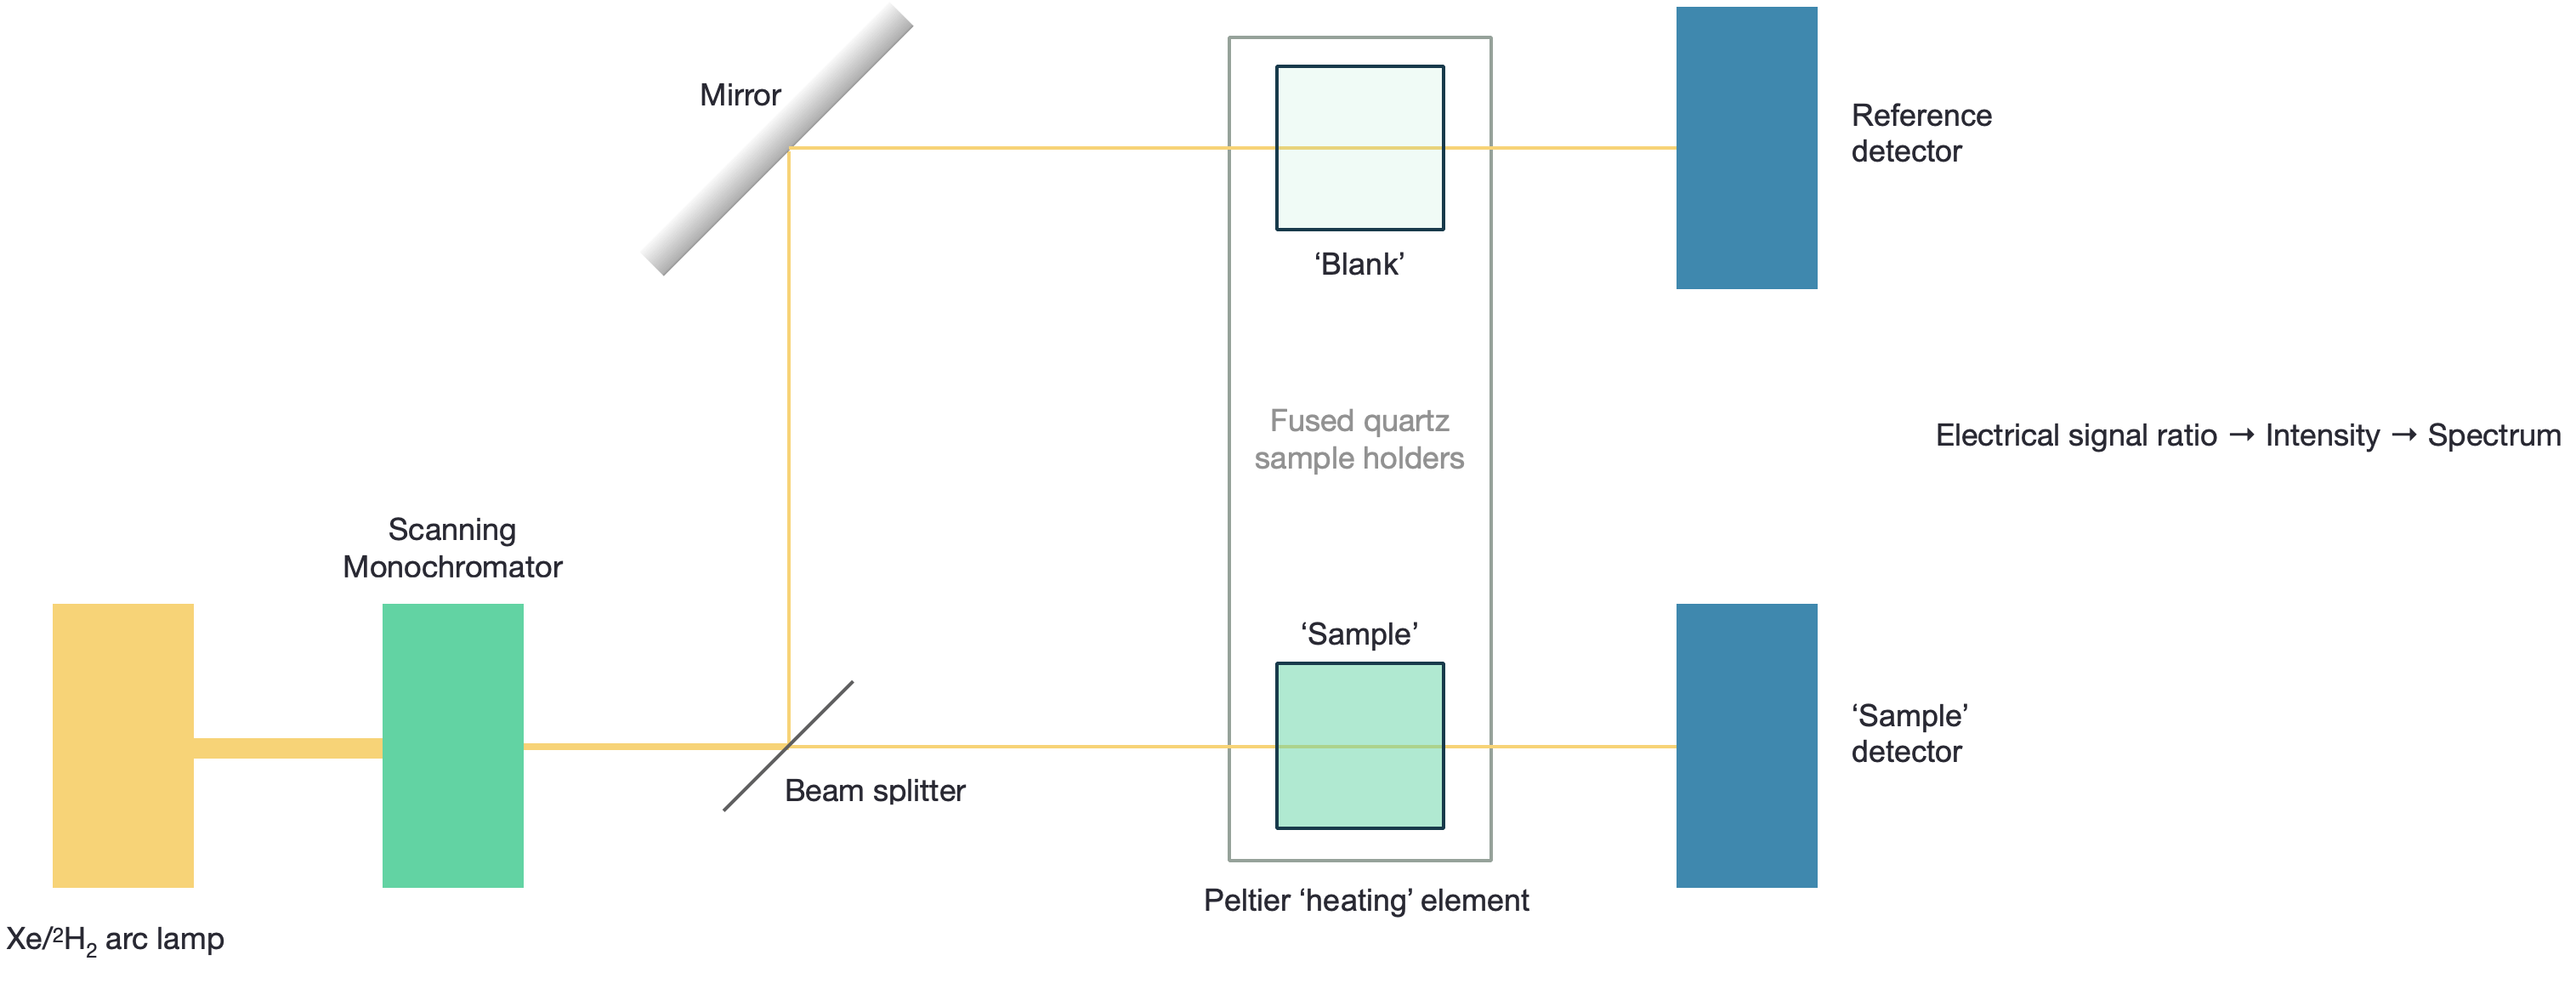
\includegraphics[width=1\linewidth]{images/UVvis} 

}

\caption{A fluorimeter consists of a source of light, wavelength selector, cell holder and detector, however, just like with UV/Vis instruments the complexity of each of these is very much dependent upon the instrument used.}\label{fig:fluorimeter}
\end{figure}

Figure \ref{fig:fluorimeter} shows the schematic of higher end fluorimeter with scanning monochromators for both the excitation and emission. Some lower end instruments may use band pass filters to select a `single' excitation (and emission) wavelength, or else use a diode as an excitation source. The university uses both of these instrument types in the teaching labs, with the diode instrument using a two dimensional echelle grating such that the full emission spectrum is recorded `instantly'. The CCD detector is considerably less sensitive than the PMT, but the cost is considerably lower and so they are used in some instruments.

\begin{figure}

{\centering 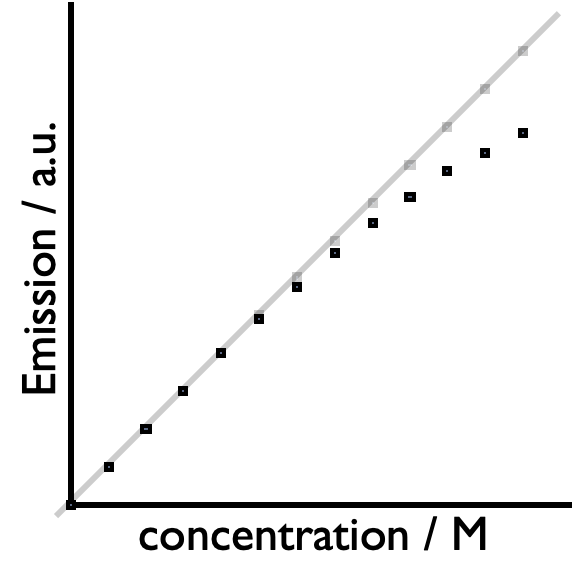
\includegraphics[width=0.4\linewidth]{images/sat} 

}

\caption{The detectors in fluorimeters may be easily saturated showing a deviation from the linear (Beer-Lambert) relationship you would expect with increasing concentration, this same effect is also seen as you increase the applied potential on the PMT or increase the slitwidth or integration time.}\label{fig:sat}
\end{figure}

The detectors in fluorescence spectrometers are easily over saturated (figure @ref\{fig:sat\}), therefore it is important to ensure that the response remains within the linear region of the instrument. To do this there are a number of ways that the signal may be reduced, these include:

\begin{itemize}
\tightlist
\item
  reducing the applied potential on the PMT
\item
  closing either the emission and/or excitation slits
\item
  reducing the concentration of the sample
\item
  reducing the path length of the sample
\item
  reducing the integration time (the time each `sample' is gathered for)
\item
  change the excitation wavelength
\end{itemize}

PMTs are less sensitive at long wavelengths and so `corrections' are usually used in this wavelength regime.

Emission light is recorded at 90º to the incident wavelength radiation to minimise optical artifacts and to separate out the emission from the intense excitation beam. The are usually scattering signals in the emission (from both Raman (inelastically scattered) and frequency halved elastic scattering) these are usually only observed at low fluorescence intensities.

\hypertarget{emission-fluorimetery}{%
\subsection{Emission fluorimetery}\label{emission-fluorimetery}}

When we are talking about fluorescence spectroscopy we are talking about emitted photons, whether they are fluorescent photons, or phosphorescent photons.

\begin{longtable}[]{@{}lll@{}}
\caption{\label{tab:phototrans} The excitation and decay pathways in molecules.}\tabularnewline
\toprule
\endhead
\begin{minipage}[t]{0.39\columnwidth}\raggedright
\emph{`Allowed transitions'}\strut
\end{minipage} & \begin{minipage}[t]{0.26\columnwidth}\raggedright
\strut
\end{minipage} & \begin{minipage}[t]{0.26\columnwidth}\raggedright
\strut
\end{minipage}\tabularnewline
\begin{minipage}[t]{0.39\columnwidth}\raggedright
Singlet-singlet absorption Singlet-singlet emission\strut
\end{minipage} & \begin{minipage}[t]{0.26\columnwidth}\raggedright
fluorescence\strut
\end{minipage} & \begin{minipage}[t]{0.26\columnwidth}\raggedright
\(S_0 + h \nu \longrightarrow S_1\) \(S_1 \longrightarrow S_0 + h \nu '\)\strut
\end{minipage}\tabularnewline
\begin{minipage}[t]{0.39\columnwidth}\raggedright
\emph{`Forbidden transitions'}\strut
\end{minipage} & \begin{minipage}[t]{0.26\columnwidth}\raggedright
\strut
\end{minipage} & \begin{minipage}[t]{0.26\columnwidth}\raggedright
\strut
\end{minipage}\tabularnewline
\begin{minipage}[t]{0.39\columnwidth}\raggedright
Singlet-triplet absorption Triplet-singlet emission\strut
\end{minipage} & \begin{minipage}[t]{0.26\columnwidth}\raggedright
phosphorescence\strut
\end{minipage} & \begin{minipage}[t]{0.26\columnwidth}\raggedright
\(S_0 + h \nu \longrightarrow T_1\) \(T_1 \longrightarrow S_0 + h \nu ''\)\strut
\end{minipage}\tabularnewline
\begin{minipage}[t]{0.39\columnwidth}\raggedright
\emph{`Other transitions'}\strut
\end{minipage} & \begin{minipage}[t]{0.26\columnwidth}\raggedright
\strut
\end{minipage} & \begin{minipage}[t]{0.26\columnwidth}\raggedright
\strut
\end{minipage}\tabularnewline
\begin{minipage}[t]{0.39\columnwidth}\raggedright
Internal conversion \strut
\end{minipage} & \begin{minipage}[t]{0.26\columnwidth}\raggedright
(vibrational relaxation) (vibrational relaxation)\strut
\end{minipage} & \begin{minipage}[t]{0.26\columnwidth}\raggedright
\(S_1 \longrightarrow S_0 + heat\) \(S_1 \longrightarrow T_1 + heat\) \(T_1 \longrightarrow S_0 + heat\)\strut
\end{minipage}\tabularnewline
\begin{minipage}[t]{0.39\columnwidth}\raggedright
\emph{Other pathways}\strut
\end{minipage} & \begin{minipage}[t]{0.26\columnwidth}\raggedright
\strut
\end{minipage} & \begin{minipage}[t]{0.26\columnwidth}\raggedright
\strut
\end{minipage}\tabularnewline
\begin{minipage}[t]{0.39\columnwidth}\raggedright
Quenching of excited state Chemistry from excited state\strut
\end{minipage} & \begin{minipage}[t]{0.26\columnwidth}\raggedright
\strut
\end{minipage} & \begin{minipage}[t]{0.26\columnwidth}\raggedright
\(S_1 + Q \longrightarrow S_0 + Q +heat\) \(S_1 + Q \longrightarrow S_0 + Q^\ast +heat\) \(T_1 + Q \longrightarrow S_0 + Q +heat\) \(T_1 + Q \longrightarrow S_0 + Q^\ast +heat\) \(S_1 \longrightarrow\) new/changed molecule\strut
\end{minipage}\tabularnewline
\bottomrule
\end{longtable}

Any process that has either emission or scattering of a photon can be seen in the fluorimeter, however scatting is usually considerably weaker and is only an issue at very low emission intensities.

When we think about fluorescence spectroscopy it is usually steady state (constant illumination)emission mode that we think of. In this technique the excitation wavelength is fixed and the emission is scanned.

It is a difficult technique to quantify, and so if comparing samples the same settings (slit width, PMT voltage, \(\lambda_{ex}\), scan rate) should be used, and the absorbance of each sample noted at \(\lambda_{ex}\).

The wavelength of emmission is calibrated using a water Raman. This is useful as it doesn't matter the purity of the water, and any excitation wavelength may be used (although if 350 nm (\(\lambda\)\textsubscript{max,em} = 397 nm) is available this is frequently used for no other reason than tradition). The Raman is an inelastic scattering and so always appears at a well defined wavelength (equation @ref\{eq:waterRaman\}).

\begin{equation}
\frac{1}{\lambda_{\textrm{em, µm}}}=\frac{1}{\lambda_{\textrm{ex, µm}}}-0.340 \textrm{ µm}^{-1}
\label{eq:waterRaman}
\end{equation}

Figure @ref\{fig:slitwidth\} shows the effect of slit width of the appearance of a water Raman calibration spectrum, the peak is Gaussian in profile and relatively intense so narrow slit widths may be used. This peak can overlay on the emission spectrum, but can manually be removed if necessary.

\begin{figure}

{\centering 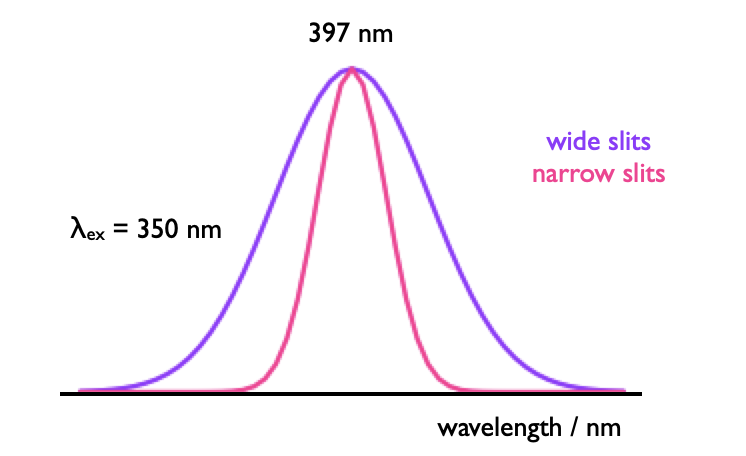
\includegraphics[width=0.4\linewidth]{images/waterRaman} 

}

\caption{The Gaussian profile of a water Raman spectrum used to calibrate the emission wavlength in fluorimeters.}\label{fig:waterRaman}
\end{figure}

Increasing the integration time improves the signal to noise ratio, but the signal only improves relative to the noise in a \(\sqrt{n}\) ratio, so as the integration time increases by four, the signal to noise ratio increases by 2.

\hypertarget{excitation-spectroscopy}{%
\subsection{Excitation spectroscopy}\label{excitation-spectroscopy}}

More on this technique will be discussed later in the course, but it is a measure of how the emission intensity varies with the excitaiton (or absorbance) of the sample - the technique can show where the excited states in a system come from.

What we do know though is that the emission intensity is very dependent upon the wavelength you excite, as the amount of absorption (and therefore excited states generated) is very dependent on wavelength (figure @ref\{fig:normabs\}).

\begin{figure}

{\centering 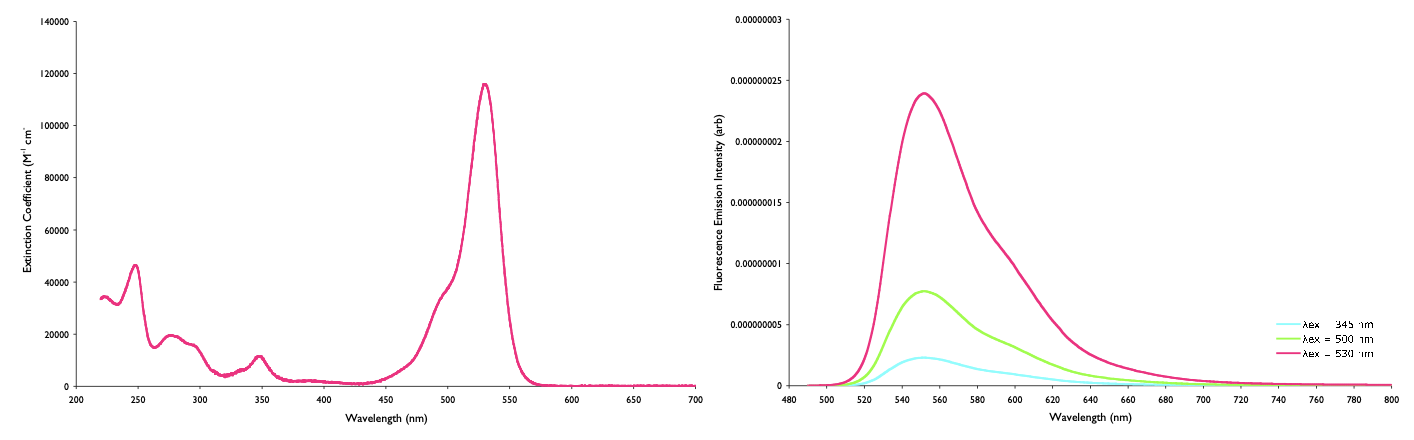
\includegraphics[width=0.4\linewidth]{images/normabs} 

}

\caption{The intensity of emission depends upon the amount of absorption at the excitation wavelength, however if each of these emission spectra, of rhodamine 6G (right), are divided by the amount of absorbance (left), then the normalised emission is the same in each case.}\label{fig:normabs}
\end{figure}

The intensity of the source varies a lot with wavelength, and so the excitation detector is used to `normalise' the emission intensity against the intensity of light generating the excited states.

\hypertarget{questions}{%
\section{Questions}\label{questions}}

\begin{enumerate}
\def\labelenumi{\arabic{enumi}.}
\tightlist
\item
  Why are emission spectra recorded at 90º to the incident light?
\end{enumerate}

\begin{enumerate}
\def\labelenumi{\alph{enumi}.}
\tightlist
\item
  emission intensity is most intense normal (at 90º) to the excitation source
\item
  90º is the best angle to separate the Raman signal from the emission signal
\item
  it is a good angle to ensure no excitation light makes it to the emission detector
\item
  it reduces the amount to reabsorption of light by minimising the path length
\item
  it maximises internal reflections, ensuring the most emission from the sample
\end{enumerate}

\begin{enumerate}
\def\labelenumi{\arabic{enumi}.}
\setcounter{enumi}{1}
\tightlist
\item
  Which of the following is not an assumption of the Beer-Lambert law?
\end{enumerate}

\begin{enumerate}
\def\labelenumi{\alph{enumi}.}
\tightlist
\item
  The absorbing molecules must be homogeneously distributed in solution
\item
  Incident radiation must be normal to the transition dipole of the molecule
\item
  The absorbers must act independently of each other
\item
  The incident radiation must be collimated (parallel rays) and pass through the same path length
\item
  The incident radiation must have a band width that is more narrow than the absorbing transition
\item
  The intensity of incident light must be low to ensure the population of an excited state is negligible
\end{enumerate}

\begin{enumerate}
\def\labelenumi{\arabic{enumi}.}
\setcounter{enumi}{2}
\tightlist
\item
  Why does a molecule absorb light; what conditions are needed?
\end{enumerate}

\begin{enumerate}
\def\labelenumi{\alph{enumi}.}
\tightlist
\item
  only the energy gap ΔE matters
\item
  only the intensity of light matters, with enough light it will always absorb
\item
  the extinction coefficient governs how much light will be absorbed
\item
  the energy gap and polarisation of the electromagnetic field matter
\item
  the solvent molecules must be aligned with the magnetic field
\item
  only the polarisation of the magnetic field matters
\end{enumerate}

\hypertarget{answers}{%
\section{Answers}\label{answers}}

\begin{enumerate}
\def\labelenumi{\arabic{enumi}.}
\tightlist
\item
  Why are emission spectra recorded at 90º to the incident light?
\end{enumerate}

\begin{enumerate}
\def\labelenumi{\alph{enumi}.}
\tightlist
\item
  emission intensity is most intense normal (at 90º) to the excitation source
\end{enumerate}

\begin{itemize}
\tightlist
\item
  Fluorescence should be isotropic in the steady state so no angle has a higher emission intensity
\end{itemize}

\begin{enumerate}
\def\labelenumi{\alph{enumi}.}
\setcounter{enumi}{1}
\tightlist
\item
  90º is the best angle to separate the Raman signal from the emission signal
\end{enumerate}

\begin{itemize}
\tightlist
\item
  Raman like emission is isotropic - the only way you can separate them is using time resolved methods, but Raman is usually considerably less intense than the emission signal.
\end{itemize}

\begin{enumerate}
\def\labelenumi{\alph{enumi}.}
\setcounter{enumi}{2}
\tightlist
\item
  { it is a good angle to ensure no excitation light makes it to the emission detector }
\end{enumerate}

\begin{itemize}
\tightlist
\item
  Incident light passes straight through, any other angle which can separate this would be fine, but 90º is usually used because of the shape of the cuvettes (square)
\end{itemize}

\begin{enumerate}
\def\labelenumi{\alph{enumi}.}
\setcounter{enumi}{3}
\tightlist
\item
  { it reduces the amount to reabsorption of light by minimising the path length}
\end{enumerate}

\begin{itemize}
\tightlist
\item
  This is called the inner filter effect - it can be a problem, and recording at 90º will minimise the path length but the best thing to do is ensure that the concentration, or intensity of incident light (slit width) is reduced
\end{itemize}

\begin{enumerate}
\def\labelenumi{\alph{enumi}.}
\setcounter{enumi}{4}
\tightlist
\item
  it maximises internal reflections, ensuring the most emission from the sample
\end{enumerate}

\begin{itemize}
\tightlist
\item
  In a square cuvette it should minimise the effect of internal reflections, this is not something we want as we are assuming the light only travels through the sample once
\end{itemize}

\begin{enumerate}
\def\labelenumi{\arabic{enumi}.}
\setcounter{enumi}{1}
\tightlist
\item
  Which of the following is not an assumption of the Beer-Lambert law?
\end{enumerate}

\begin{enumerate}
\def\labelenumi{\alph{enumi}.}
\tightlist
\item
  The absorbing molecules must be homogeneously distributed in solution
\item
  { Incident radiation must be normal to the transition dipole of the molecule }
\end{enumerate}

\begin{itemize}
\tightlist
\item
  This statement is the exact opposite of being homogeneously distributed, only molecules with the transition dipole moment aligned correctly will absorb, but it shouldn't be that all molecules are aligned
\end{itemize}

\begin{enumerate}
\def\labelenumi{\alph{enumi}.}
\setcounter{enumi}{2}
\tightlist
\item
  The absorbers must act independently of each other
  d.The incident radiation must be collimated (parallel rays) and pass through the same path length
\item
  The incident radiation must have a band width that is more narrow than the absorbing transition
\item
  The intensity of incident light must be low to ensure the population of an excited state is negligible
\end{enumerate}

\begin{enumerate}
\def\labelenumi{\arabic{enumi}.}
\setcounter{enumi}{2}
\tightlist
\item
  Why does a molecule absorb light; what conditions are needed?
\end{enumerate}

\begin{enumerate}
\def\labelenumi{\alph{enumi}.}
\tightlist
\item
  only the energy gap ΔE matters
\end{enumerate}

\begin{itemize}
\tightlist
\item
  It matters, it isn't the only thing\ldots{}
\end{itemize}

\begin{enumerate}
\def\labelenumi{\alph{enumi}.}
\setcounter{enumi}{1}
\tightlist
\item
  only the intensity of light matters, with enough light it will always absorb
\end{enumerate}

\begin{itemize}
\tightlist
\item
  Nope\ldots{} more power doesn't work, although you can get some cool non-linear two photon effects with enough power it still has to be the right energy
\end{itemize}

\begin{enumerate}
\def\labelenumi{\alph{enumi}.}
\setcounter{enumi}{2}
\tightlist
\item
  the extinction coefficient governs how much light will be absorbed
\end{enumerate}

\begin{itemize}
\tightlist
\item
  Yes, but it isn't a condition required
\end{itemize}

\begin{enumerate}
\def\labelenumi{\alph{enumi}.}
\setcounter{enumi}{3}
\tightlist
\item
  { the energy gap and polarisation of the electromagnetic field matter }
\end{enumerate}

\begin{itemize}
\tightlist
\item
  Yes the energy gap (wavelength) needs to be appropriate, but the transition dipole moment of that transition of the chromophore must be aligned with the polarisation of the EM light
\end{itemize}

\begin{enumerate}
\def\labelenumi{\alph{enumi}.}
\setcounter{enumi}{4}
\tightlist
\item
  the solvent molecules must be aligned with the magnetic field
\end{enumerate}

\begin{itemize}
\tightlist
\item
  The solvent has nothing to do with the transition dipole, it may affect ΔE
\end{itemize}

\begin{enumerate}
\def\labelenumi{\alph{enumi}.}
\setcounter{enumi}{5}
\tightlist
\item
  only the polarisation of the magnetic field matters
\end{enumerate}

\begin{itemize}
\tightlist
\item
  Again, it matters that the transition dipole moment and the polarisation of light are matched but for UV/Vis the incident light should be unpolarised
\end{itemize}

\hypertarget{ch:LDCD}{%
\chapter{LD (linear dichroism) and CD (circular dichroism)}\label{ch:LDCD}}

\hypertarget{sec:LD}{%
\section{Linear dichroism}\label{sec:LD}}

If we consider the Beer-Lambert law, we have previously said that one of the assumptions of this law is that absorbers are distributed randomly in solution\ldots{} however, when we look at dichroism techniques, they are actively looking at only exciting molecules aligned with the polarisation.

You will recall that light is only absorbed by a molecule when the polarisation of the light is aligned with the transition dipole moment.

Light is only absorbed by a molecule if the polarisation of the light aligns with the transition dipole moment on the molecule. Figure \ref{fig:CS2} shows CS\textsubscript{2} a simple linear molecule - where the transition dipole moment runs along the long axis of the molecule.

\begin{figure}

{\centering 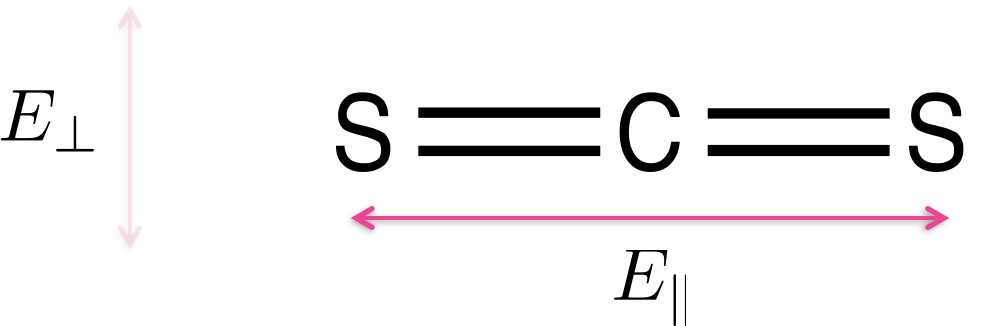
\includegraphics[width=0.6\linewidth]{images/CS2} 

}

\caption{Carbon disulfide (CS~2~) is a linear molecule -  due to the shape of the molecule there is a transition dipole which runs down the length of the long axis. Light aligned such that the electric field runs parallel with the long axis of the molecule E~||~ will be absorbed, light which in which the electric field runs perpendicular to the long axis of the molecule E~⊥~ will not be absorbed.}\label{fig:CS2}
\end{figure}

For more complicated molecules each of the transitions from the HOMO, HOMO-1 to the LUMO \emph{etc.} occur with different transition dipole moments across the chromophore, figure @ref\{fig:adenosine\}. Each transition is only excited when light is aligned with that transition; in most cases this isn't something we need to consider as most incident light we consider is isotropic, but alignment of transition dipoles (either between light and molecules - or between two different molecules) is an important consideration.

\begin{figure}

{\centering 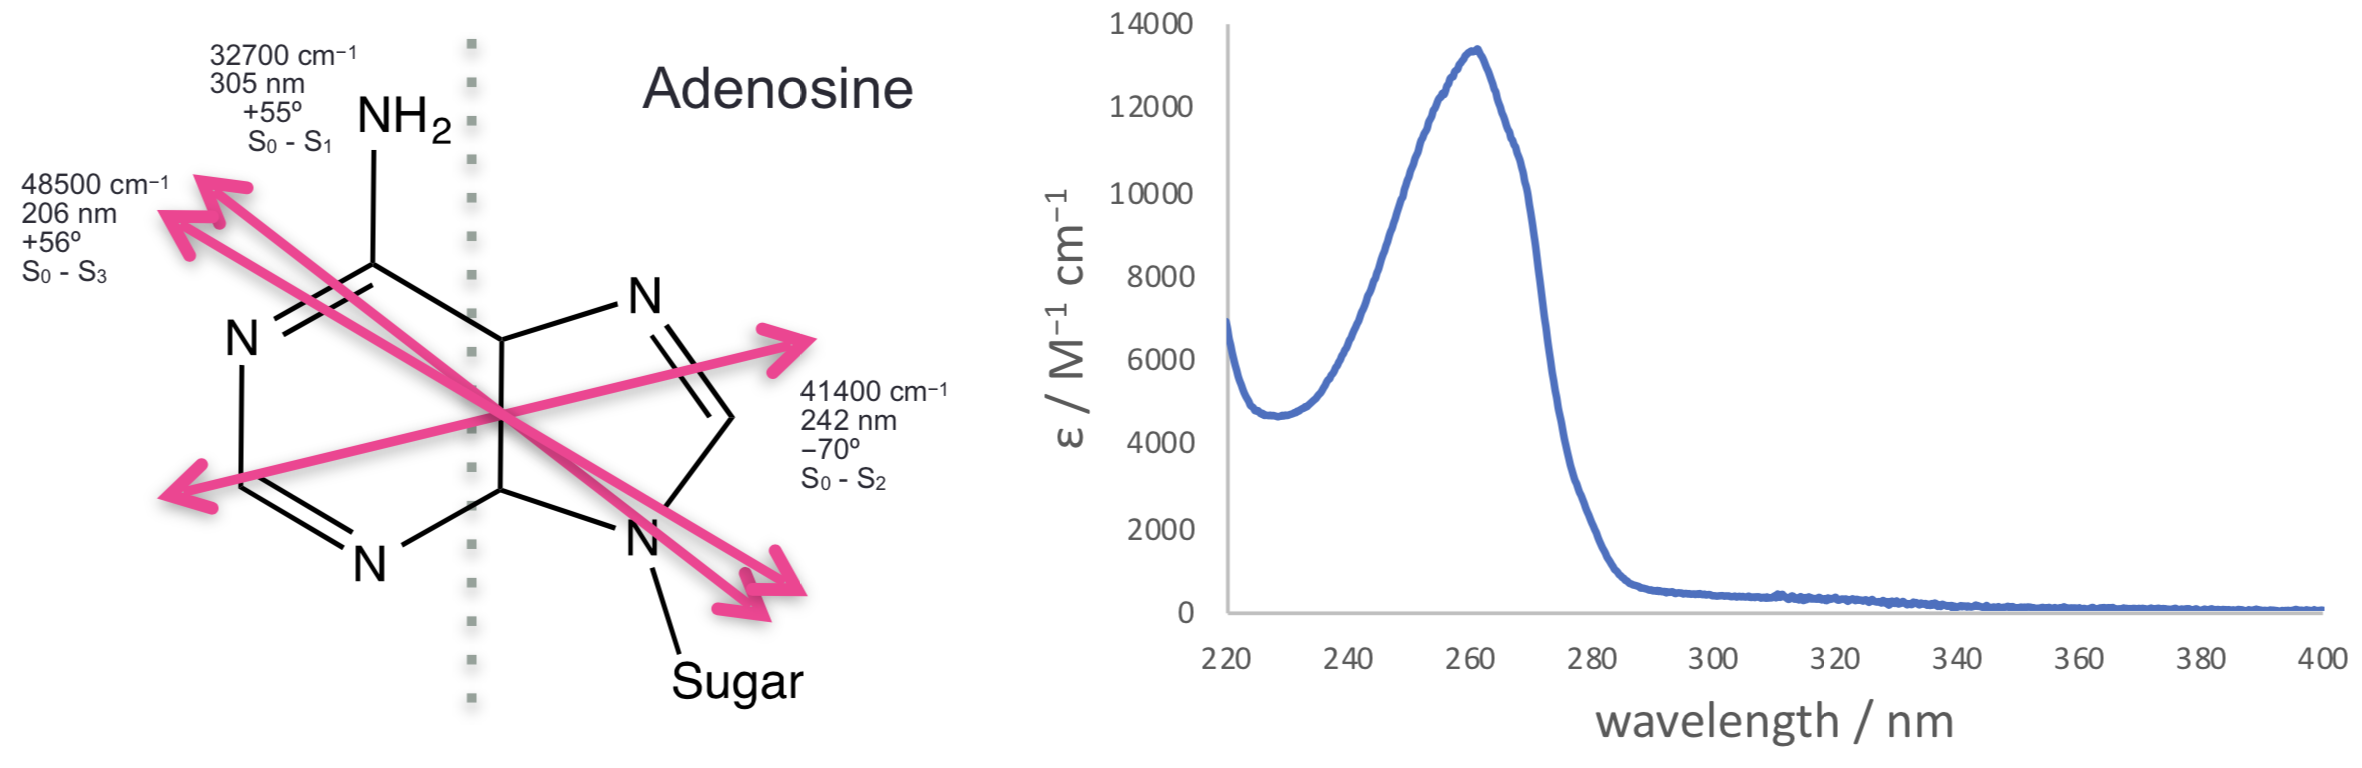
\includegraphics[width=1\linewidth]{images/adenosine} 

}

\caption{The three lowest energy transitions of adenosine each indicated with their transition dipole moment (all in the plane of the molecule, calculated values).These match with the observed spectrum with a weak transition around 310 nm, a much stronger transition around 260 nm and a third transition starting at the edge of the measured spectrum. Spectrum Adapted from OMLC ( https:// omlc.org/spectra/PhotochemCAD/html/033.html), 31st October 2018}\label{fig:adenosine}
\end{figure}

As already discussed the transition dipole moment is derived from the difference in electron density of the ground and excited state.

Linear dichroism uses linearly polarised light and is a measure of the difference in absorbance of the sample between plane polarised light parallel and perpendicular to a reference axis (equation \eqref{eq:LD}, figure \ref{fig:LD}).

\begin{equation}
LD = A_{\parallel} - A_{\perp}
\label{eq:LD}
\end{equation}

\begin{figure}

{\centering 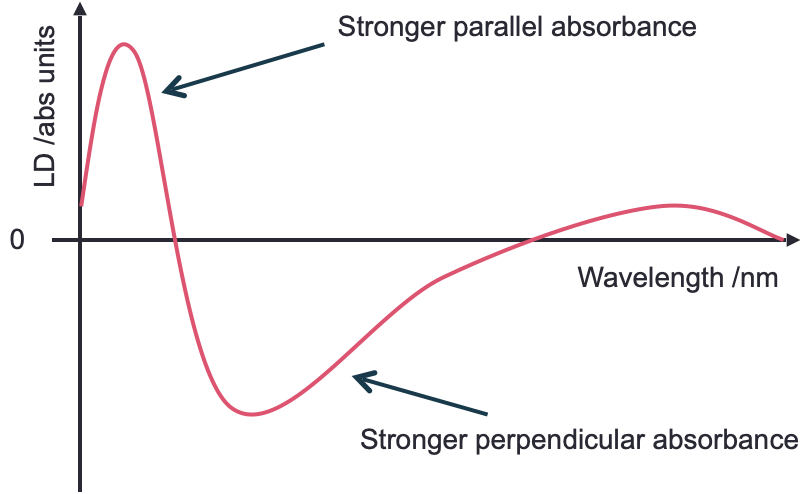
\includegraphics[width=0.6\linewidth]{images/LD} 

}

\caption{A generic LD spectrum to illustrate features of a sample with regions of the spectrum showing a postive LD. An isotropic sample would show 0 LD.}\label{fig:LD}
\end{figure}

So if we consider a simple molecular system, that of CS\textsubscript{2} (figure \ref{fig:CS2}, then light which is polarised in alignment with the long axis of the molecule, \(E_{\parallel}\), (which is aligned with the transition dipole moment on the molecule) will be absorbed, whereas light normal to this, \(E_{perp}\), will be transmitted as light is passed through the sample. Our dichroism, \(LD\), is the difference between these two absorbance values.

This is how polaroid film works where there is a large transition dipole moment along one axis, and a negligable transition dipole along the orthoganol axis.

Adenosine (figure \ref{fig:adenosine}) is a more typical example, this is an example of a molecule with different transition dipole moments, each with a particular energy and polarisation. We can observe that the different dipole moments absorb more strongly at if we can allign our structure somehow, like in a crystal\ldots{}

We can relate the linear dichroism to the angle from the reference axis as follows (equation @ref:LDiso):

\begin{equation}
LD = \frac{3}{2}A_{\textrm{iso}}S(3 \cos^2 \alpha - 1)
\label{eq:LDiso}
\end{equation}

The reduced LD, \(LD^r\) is often used as it is concentration indpendent and so differences in the spectrum are easily observed:

\begin{equation}
LD = \frac{A_{\parallel} - A_{\perp}}{A_\textrm{iso}} \frac{3}{2}S(3 \cos^2 \alpha - 1)
\label{eq:LDred}
\end{equation}

The LD spectrophotometer looks a lot like the UV/vis (figure \ref{fig:LDspec}), however we need to add a two position polarising filter (horizontal and vertical), again just like with the UV there is a blank path (or a dummy blank path and a chopper), with similar light sources to the UV/vis (Xe arc and \textsuperscript{2}D\textsubscript{2} arc), with the detector again usually being a photodiode.

\begin{figure}

{\centering 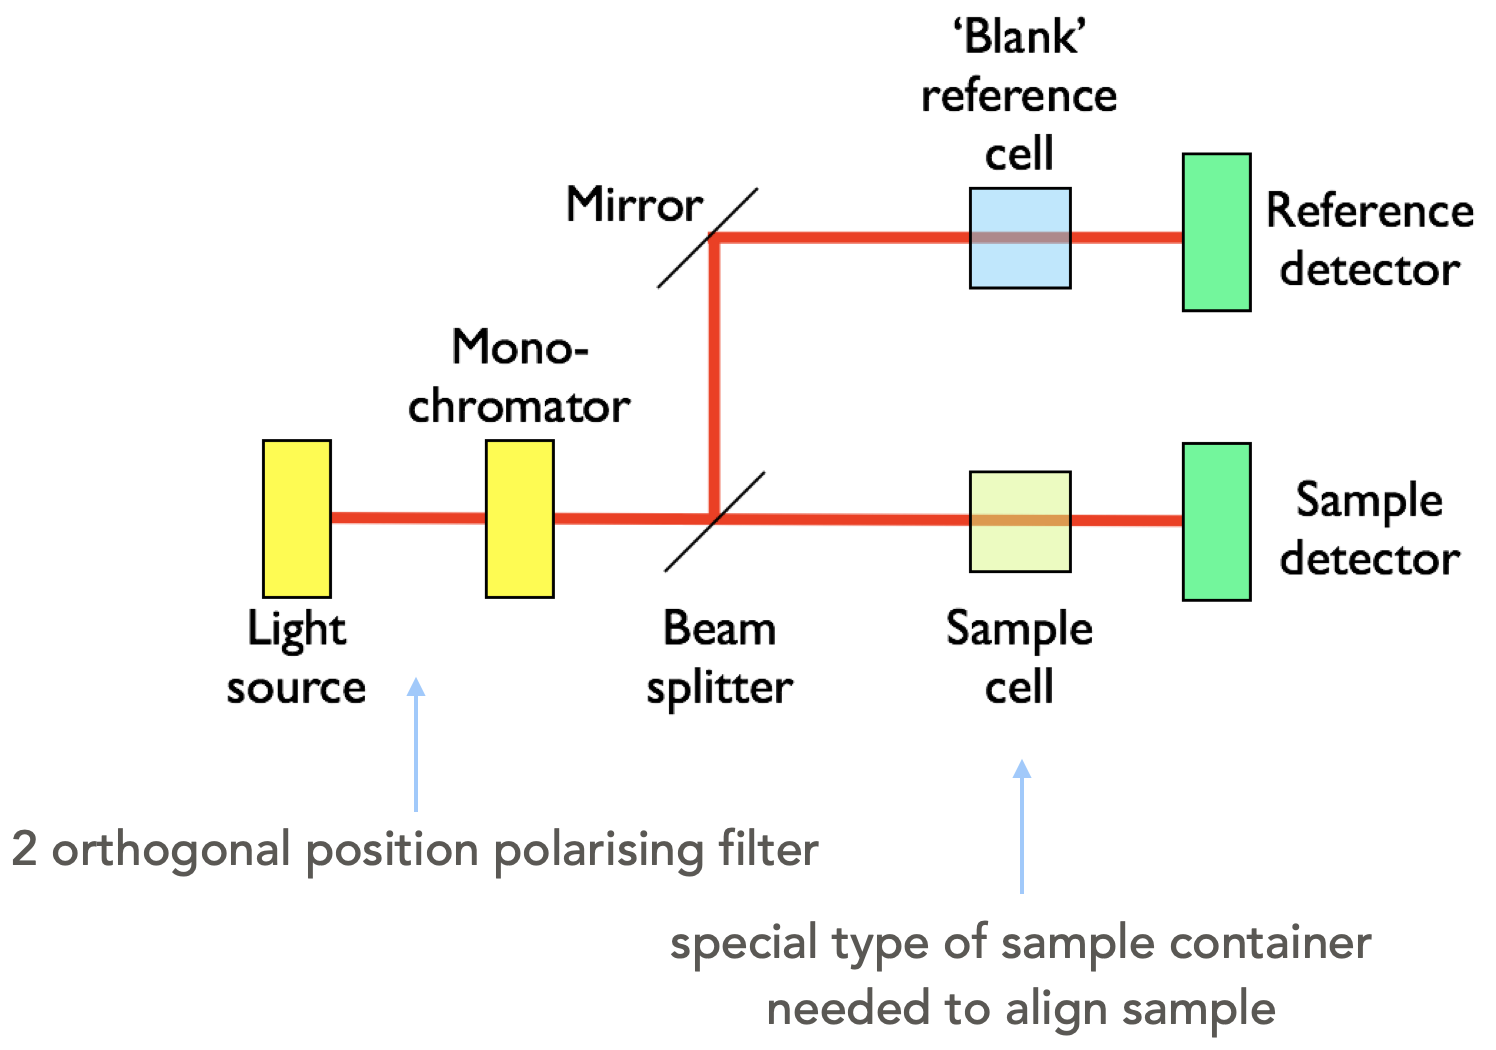
\includegraphics[width=0.6\linewidth]{images/LDspec} 

}

\caption{A block diagram of a LD spectrometer including the two position polarising filter.}\label{fig:LDspec}
\end{figure}

If the sample is solution based it will be isotropic unless there is something to help align the molecules, and consequently there will be no LD signal detected. Consequently there needs to be some form of smple alignment, which is usually achieved in one of two methods (figure @ref\{fig:LDcell\}):

\begin{itemize}
\tightlist
\item
  small molecules are embedded in a polymer film, which is then stretched in a single direction, this then coaligns the small molecules along the direction of the stretch
\item
  large molecules (such as polymers, DNA and proteins) can be aligned \emph{via} laminar flow. In this case the cuvette is a hollow cylinder with an internal bar which rotates rapidly, this causes laminar flow
\end{itemize}

\begin{figure}

{\centering 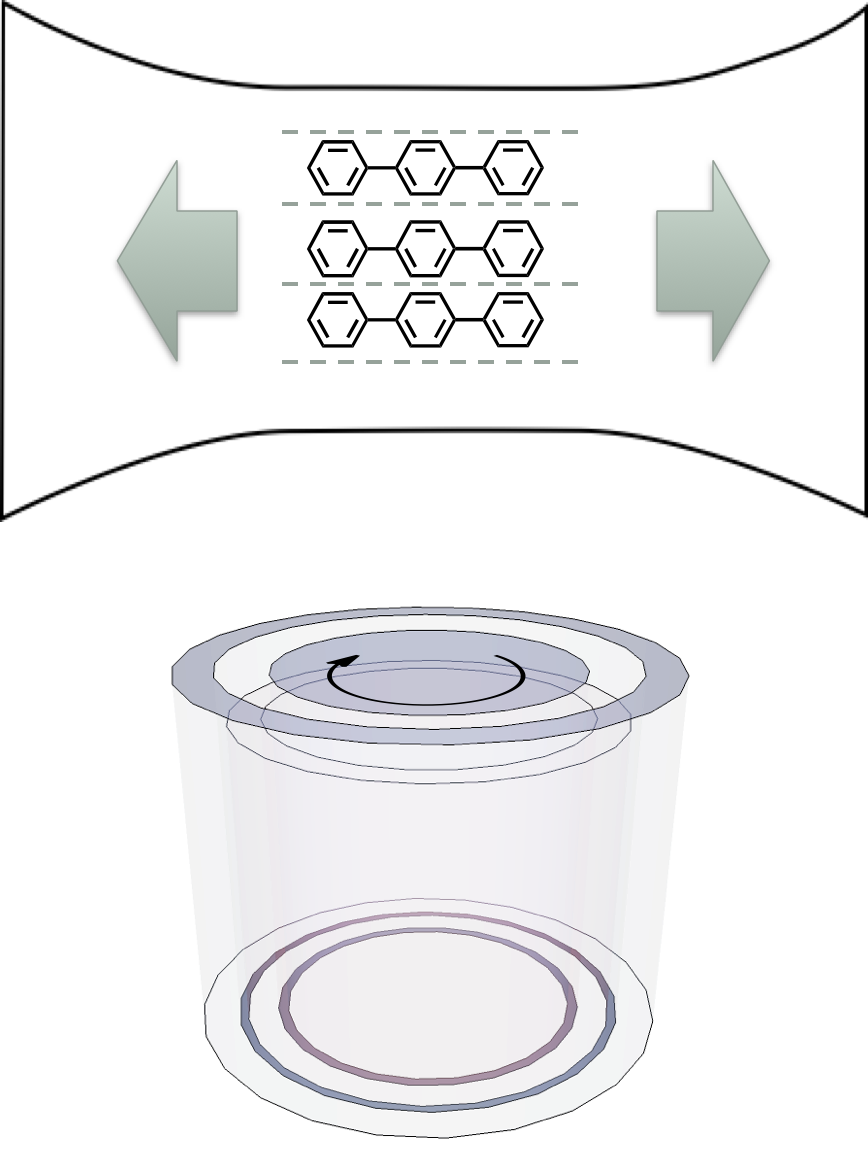
\includegraphics[width=0.6\linewidth]{images/LDcell} 

}

\caption{In order to show an LD signal there needs to be some alignment of the molecules, two methods are usually used, embedding the molecules in a polymer film and stretching the film, such that the molecules are pulled into alignment (top), or laminar flow, whereby a thin film of solvent is rapidly stired and the molecules align with this flow (like stirring spagetti (bottom)}\label{fig:LDcell}
\end{figure}

\hypertarget{circular-dichroism}{%
\section{Circular Dichroism}\label{circular-dichroism}}

Circular dichroism uses circularly polarised light and looks at the difference between the absorption of left and right hand polarised light. It is much like the use of polarimetry to look at R- and S- enantiomers, but we are combining it with UV, in that a spectrum is scanned and the CD measured over a range of wavelengths.

An excel resource has been provided on moodle (under `Other Resources') to try to help you understand how two plane waves may be combined to generate circularly polarised light.

To generate circularly polarised light two orthogonal paths of monochromatic light is passed through a birefringent material (a material with two different refractive indicies depending on the crystal plane). This retards one wave more than the other and when they combine they are out of phase and so combine to form circularly or eliptically polarised light. Calcite is an example of a birefringent material.

The phase offset will depend upon the thickness of the waveplate, the thickness of this plate can be changed by applying an alternating current causing a change in crystal shape due to teh piezoelectric effect. The bigger the potential difference the bigger the change in the size of the crystal, consequently the crystal can always be adjusted (no matter the wavelength) so that the resultant waves are always π/2 (for a quarter wave plate), or π (for a half wave plate) different in phase. This crystal oscillation is caused by a device called the photoelastic modulator.

\begin{figure}

{\centering 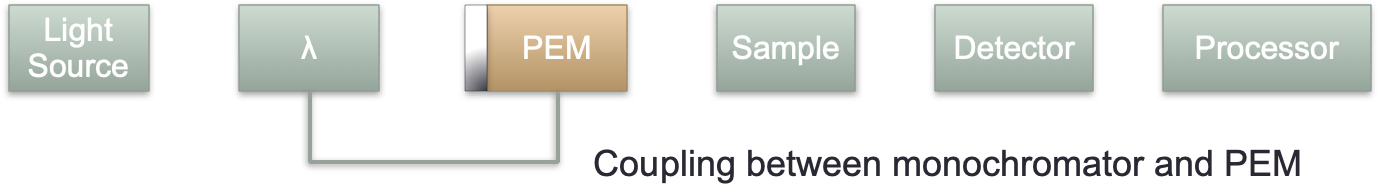
\includegraphics[width=0.6\linewidth]{images/CD} 

}

\caption{A block diagram of a CD spectrometer including the coupled monochromator and photoelastic modulator.}\label{fig:CD}
\end{figure}

In each 50 Hz cycle we get a measurement of -λ/4 (L) and +λ/4 (R) light. After passing through a sample the R \& L circularly polarised light become eliptical (and when we deconvolute the horizontal and vertical waves are no longer of equal amplitude) these combine to give the CD (equation \ref{fig:CD}).

\begin{equation}
CD = A_{\textrm{L}} - A_{\textrm{R}}
\label{eq:CD}
\end{equation}

It should be noted that there is a difference of opinion as to what reference frame constitutes left and right as far as the polarisation of light goes, papers will always state their convention.

\hypertarget{induced-dichroism}{%
\section{Induced Dichroism}\label{induced-dichroism}}

Some molecules may themselves not show either LD or CD themselves, but they may have induced dichroism because they are bound to a molecule which does.

\begin{figure}

{\centering 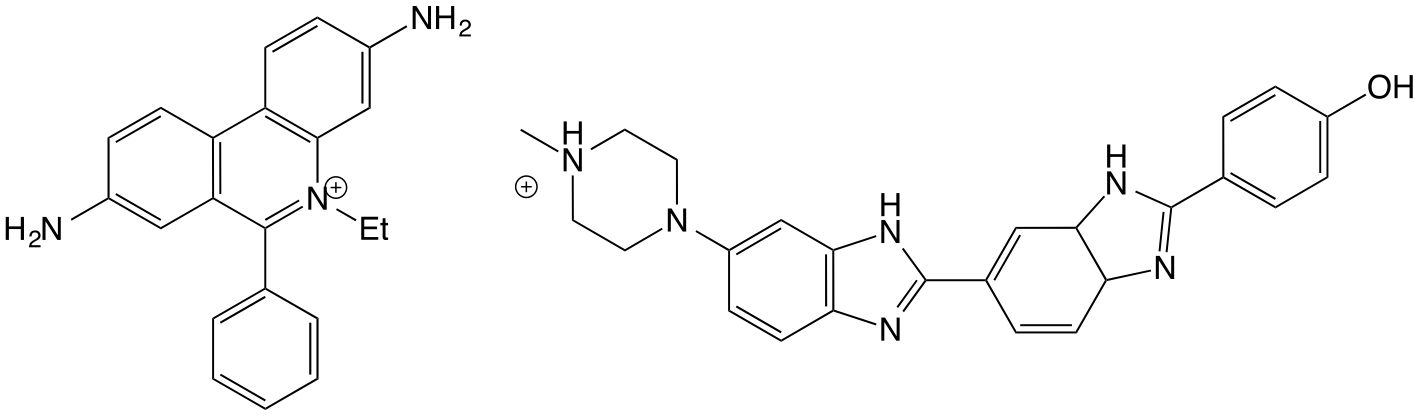
\includegraphics[width=0.6\linewidth]{images/DNAbinders} 

}

\caption{The DNA binders ethidium bromide (left) which intercalates between the base pairs of DNA, and Hoechst 33258 (right) which binds in the minor groove of DNA, by curving around the tertiary structure}\label{fig:DNAbinders}
\end{figure}

An example of this would be small dye molecules such as YO-Pro-1 (see photochemisry notes and the later workshop materials, and those listed in figure \ref{fig:DNAbinders} which is a small fluorescent dye molecule which binds to DNA. This molecule itself is achrial, and if introduced into LD with laminar flow is too small to align and so the LD should also be zero. However, when bound to DNA both an LD and CD is observed from the sample because it is now in an environment big enough to align with the laminar flow, and the DNA tertiary structure is chiral and so the dye is binding into a chrial environment and therefore an induced CD is also observed.

For induced LD, if the molecule remains in free solution the transition dipoles are aligned isotopically and no LD is observed. However if we look at binding to DNA as an example, if the molecule intercalates the transition dipole moment will be \emph{more} aligned to be perpendicular to the long axis of the molecule and will therefore display a negative LD. If the molecule has a transition dipole moment principally aligned with the long axis of the molecule then it will display a positive LD (figure \ref{fig:inducedLD}.

We can determine the binding angle (with a few added assumptions) by using equation \eqref{eq:LDiso}.

\begin{figure}

{\centering 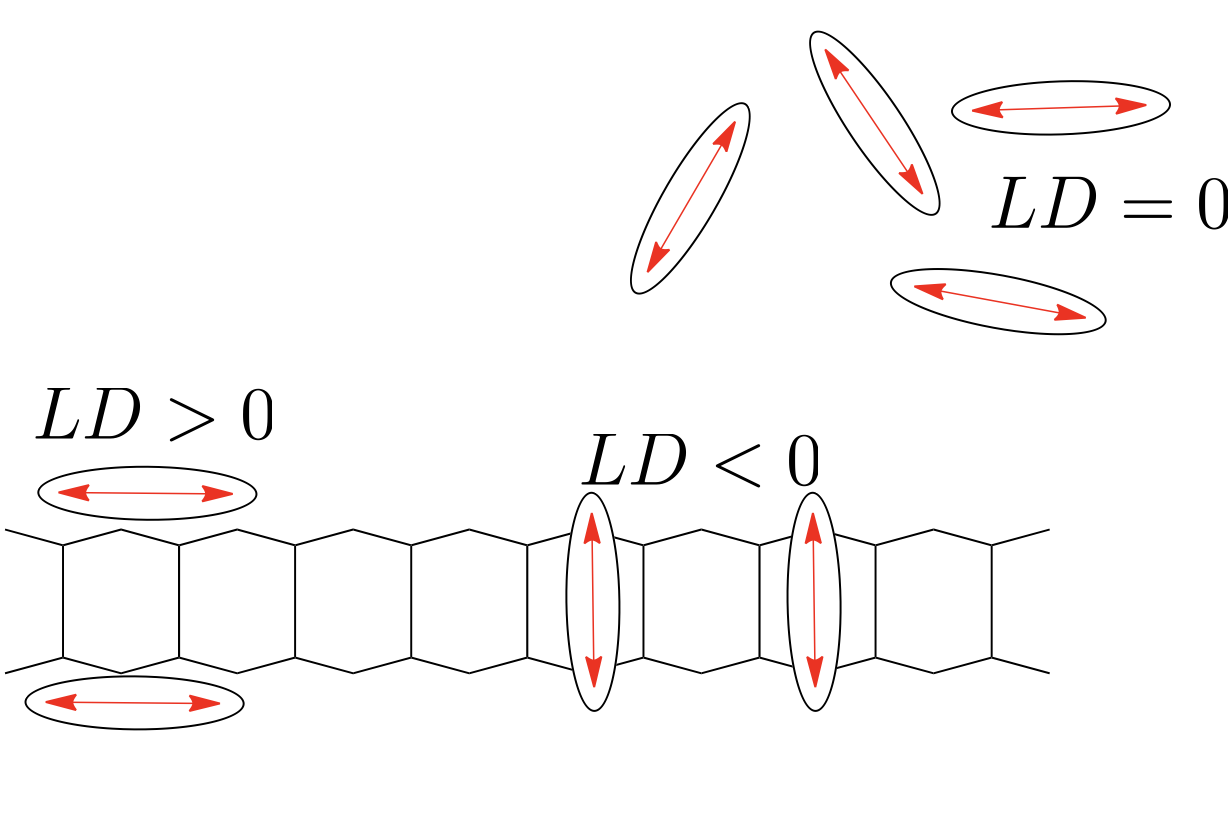
\includegraphics[width=0.6\linewidth]{images/inducedLD} 

}

\caption{Small molecules under laminar flow are too small to align and so they are aranged isotropically and therefore no LD is observed, however on binding to macromolecules such as DNA the species display an induced LD}\label{fig:inducedLD}
\end{figure}

CD may show `unwinding' (less chirality in the sample) indicating an intercalation of a molecule between the bases of DNA.

Behaviour like this can tell us a lot about drugs binding to biological molecules, in a manner which is relatively quick and simple.

\hypertarget{workshop-task}{%
\section{Workshop task}\label{workshop-task}}

You will find some slides containing absorbance, LD and CD of YO-Pro-1 and it's dimer YOYO-1 on Moodle under the CD and LD, alongside these are some questions I want you to think about and answer when looking at the spectra. You should think about general trends and not be too hung up about individual spectra.

When we meet in our next LOIL we will discuss this case study and I will be breaking you into your selected (or assigned) break out groups to discuss our ideas further, we will then wrap up the session with you sharing your group thoughts (so think about nominating a spokesperson).

I do not expect you to know a lot about DNA, just know the following:
- DNA has a negatively charged backbone
- By intercalating between the basepais the DNA has to stretch (get longer) and unwind slighly
- A helix repeats about once every 10 bases, with the bases separated by the van der Waals distance (3.4 Å)
- The bases are about about 86º to the long axis of the molecule

\hypertarget{questions}{%
\section{Questions}\label{questions}}

These questions can be used to check your understanding of the material, beware I periodically include star trek inspired technobabble in the distractors\ldots{}

\begin{enumerate}
\def\labelenumi{\arabic{enumi}.}
\item
  If a molecule is illuminated with polarised light, for it to absorb light:

  \begin{enumerate}
  \def\labelenumii{\alph{enumii}.}
  \tightlist
  \item
    only the energy gap ΔE matters
  \item
    only the intensity of light matters, with enough light it will always absorb
  \item
    the extinction coefficient governs how much light will be absorbed
  \item
    the energy gap and the orientation of the transition dipole moment matter
  \item
    the solvent molecules must be aligned with the magnetic field
  \item
    only the polarisation of the magnetic field matters
  \end{enumerate}
\item
  For a molecule to display CD absorption then:
\end{enumerate}

\begin{enumerate}
\def\labelenumi{\alph{enumi}.}
\tightlist
\item
  it must first be excited with polarised light
\item
  it must be able to be aligned with the electric field
\item
  it must have an inversion centre, i
\item
  the instantaneous transition dipole moment must be circularly polarised
\item
  the molecule must display a quadrupole in both magnetic and electric fields
\item
  there must be chirality in the molecule
\end{enumerate}

\begin{enumerate}
\def\labelenumi{\arabic{enumi}.}
\setcounter{enumi}{2}
\tightlist
\item
  For a chromophore to display induced CD absorption then:
\end{enumerate}

\begin{enumerate}
\def\labelenumi{\alph{enumi}.}
\tightlist
\item
  there must be a strong matrix coupling element between the chromophore and the molecule to which it is binding
\item
  the chromophore must have a chiral centre
\item
  the instantaneous dipole on the chromophore must interact with the electric field of the molecule to which it is binding
\item
  the absorption wavelengths of both the chromophore and chiral molecule must overlap
\item
  there must be a strong overlap integral between the emission of the chiral molecule and the absorption of the molecule to which it is binding
\item
  it must be free in solution
\item
  the chromophore must be bound in such a way to a chiral molecule that it takes on chiral optical properties
\end{enumerate}

\begin{enumerate}
\def\labelenumi{\arabic{enumi}.}
\setcounter{enumi}{3}
\tightlist
\item
  If a molecule has an absorbance and LD as shown below then:
\end{enumerate}

\begin{figure}

{\centering 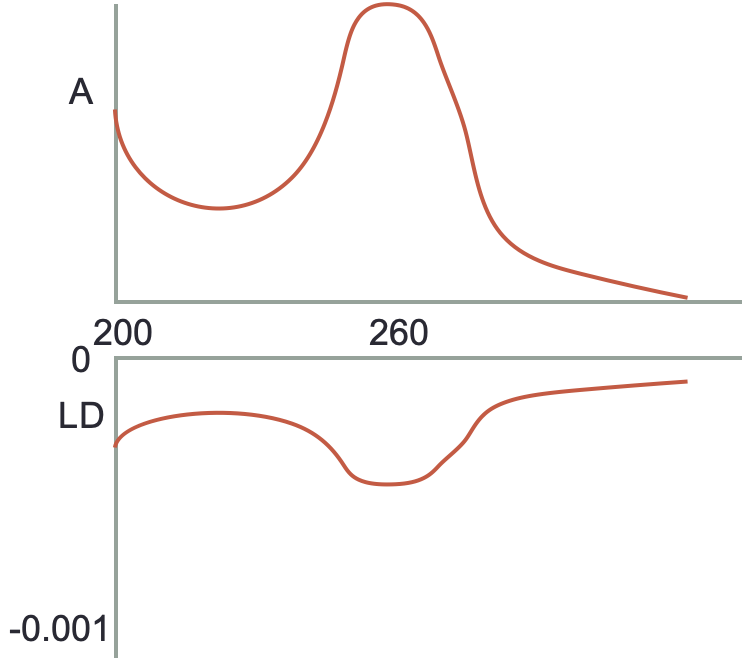
\includegraphics[width=0.6\linewidth]{images/LDquestion} 

}

\caption{Isotopic absorbance (top) and LD (bottom)}\label{fig:LDquestion}
\end{figure}

\begin{enumerate}
\def\labelenumi{\alph{enumi}.}
\tightlist
\item
  the molecule is isotropically distributed in solution
\item
  there is only a single transition within the molecule
\item
  the molecule is principally aligned parallel to the plane of polarised light
\item
  the molecule is principally aligned perpendicular to the plane of polarised light
\item
  the transition moments are aligned more parallel to the plane of polarised light
\item
  the transition moments are aligned more perpendicular to the plane of polarised light
\item
  the sample is degrading under UV light
\end{enumerate}

\hypertarget{answers}{%
\section{Answers}\label{answers}}

\begin{enumerate}
\def\labelenumi{\arabic{enumi}.}
\tightlist
\item
  If a molecule is illuminated with polarised light, for it to absorb light:
\end{enumerate}

\begin{enumerate}
\def\labelenumi{\alph{enumi}.}
\tightlist
\item
  only the energy gap ΔE matters
\end{enumerate}

\begin{itemize}
\tightlist
\item
  Again, it matters, it isn't the only thing\ldots{}
\end{itemize}

\begin{enumerate}
\def\labelenumi{\alph{enumi}.}
\setcounter{enumi}{1}
\tightlist
\item
  only the intensity of light matters, with enough light it will always absorb
\end{enumerate}

\begin{itemize}
\tightlist
\item
  Still not true
\end{itemize}

\begin{enumerate}
\def\labelenumi{\alph{enumi}.}
\setcounter{enumi}{2}
\tightlist
\item
  the extinction coefficient governs how much light will be absorbed
\end{enumerate}

\begin{itemize}
\tightlist
\item
  It does, but it isn't what matters most it just says how much light will be absorbed
\end{itemize}

\begin{enumerate}
\def\labelenumi{\alph{enumi}.}
\setcounter{enumi}{3}
\tightlist
\item
  the energy gap and the orientation of the transition dipole moment matter
\end{enumerate}

\begin{itemize}
\tightlist
\item
  This is the one
\end{itemize}

\begin{enumerate}
\def\labelenumi{\alph{enumi}.}
\setcounter{enumi}{4}
\tightlist
\item
  the solvent molecules must be aligned with the magnetic field
\end{enumerate}

\begin{itemize}
\tightlist
\item
  Still drivel
\end{itemize}

\begin{enumerate}
\def\labelenumi{\alph{enumi}.}
\setcounter{enumi}{5}
\tightlist
\item
  only the polarisation of the magnetic field matters
\end{enumerate}

\begin{itemize}
\tightlist
\item
  This time this one matters, but it isn't the only thing\ldots{}
\end{itemize}

\begin{enumerate}
\def\labelenumi{\arabic{enumi}.}
\setcounter{enumi}{1}
\tightlist
\item
  For a molecule to display CD absorption then:
\end{enumerate}

\begin{enumerate}
\def\labelenumi{\alph{enumi}.}
\tightlist
\item
  it must first be excited with polarised light
\end{enumerate}

\begin{itemize}
\tightlist
\item
  If it was first excited with polarised light we would be looking at a transient species not the ground state
\end{itemize}

\begin{enumerate}
\def\labelenumi{\alph{enumi}.}
\setcounter{enumi}{1}
\tightlist
\item
  it must be able to be aligned with the electric field
\end{enumerate}

\begin{itemize}
\tightlist
\item
  For a molecule to absorb there must be alignment of the transition dipole moment with the incident light, but nothing in particular with the CD is unique
\end{itemize}

\begin{enumerate}
\def\labelenumi{\alph{enumi}.}
\setcounter{enumi}{2}
\tightlist
\item
  it must have an inversion centre, i
\end{enumerate}

\begin{itemize}
\tightlist
\item
  If a molecule has an inversion centre it is NOT chiral
\end{itemize}

\begin{enumerate}
\def\labelenumi{\alph{enumi}.}
\setcounter{enumi}{3}
\tightlist
\item
  the instantaneous transition dipole moment must be circularly polarised
\end{enumerate}

\begin{itemize}
\tightlist
\item
  Ooooh-oooooooooh-oh-oh-oh-oh-oooooh the gibberish star trek answer
\end{itemize}

\begin{enumerate}
\def\labelenumi{\alph{enumi}.}
\setcounter{enumi}{4}
\tightlist
\item
  the molecule must display a quadrupole in both magnetic and electric fields
\end{enumerate}

\begin{itemize}
\tightlist
\item
  Ooooh-oooooooooh-oh-oh-oh-oh-oooooh the gibberish star trek answer - oooh two!
\end{itemize}

\begin{enumerate}
\def\labelenumi{\alph{enumi}.}
\setcounter{enumi}{5}
\tightlist
\item
  there must be chirality in the molecule
\end{enumerate}

\begin{itemize}
\tightlist
\item
  Yup - CD only works with chiral molecules (or molecules in a chiral environment (induced CD))
\end{itemize}

\begin{enumerate}
\def\labelenumi{\arabic{enumi}.}
\setcounter{enumi}{2}
\tightlist
\item
  For a chromophore to display induced CD absorption then:
\end{enumerate}

\begin{enumerate}
\def\labelenumi{\alph{enumi}.}
\tightlist
\item
  there must be a strong matrix coupling element between the chromophore and the molecule to which it is binding
\end{enumerate}

\begin{itemize}
\tightlist
\item
  Ooooh-oooooooooh-oh-oh-oh-oh-oooooh the gibberish star trek answer
\end{itemize}

\begin{enumerate}
\def\labelenumi{\alph{enumi}.}
\setcounter{enumi}{1}
\tightlist
\item
  the chromophore must have a chiral centre
\end{enumerate}

\begin{itemize}
\tightlist
\item
  This will display CD not induced CD
\end{itemize}

\begin{enumerate}
\def\labelenumi{\alph{enumi}.}
\setcounter{enumi}{2}
\tightlist
\item
  the instantaneous dipole on the chromophore must interact with the electric field of the molecule to which it is binding
\end{enumerate}

\begin{itemize}
\tightlist
\item
  This would be a dipole induced dipole interaction - back to first year bonding theory
\end{itemize}

\begin{enumerate}
\def\labelenumi{\alph{enumi}.}
\setcounter{enumi}{3}
\tightlist
\item
  the absorption wavelengths of both the chromophore and chiral molecule must overlap
\end{enumerate}

\begin{itemize}
\tightlist
\item
  No reason for this to be true, if they are it would just complicate the spectrum
\end{itemize}

\begin{enumerate}
\def\labelenumi{\alph{enumi}.}
\setcounter{enumi}{4}
\tightlist
\item
  there must be a strong overlap integral between the emission of the chiral molecule and the absorption of the molecule to which it is binding
\end{enumerate}

\begin{itemize}
\tightlist
\item
  Nope, no reason for this to be true
\end{itemize}

\begin{enumerate}
\def\labelenumi{\alph{enumi}.}
\setcounter{enumi}{5}
\tightlist
\item
  it must be free in solution
\end{enumerate}

\begin{itemize}
\tightlist
\item
  No induced CD if free in solution
\end{itemize}

\begin{enumerate}
\def\labelenumi{\alph{enumi}.}
\setcounter{enumi}{6}
\tightlist
\item
  the chromophore must be bound in such a way to a chiral molecule that it takes on chiral optical properties
\end{enumerate}

\begin{itemize}
\tightlist
\item
  Yes the chiral choromophore must be in a chiral environment
\end{itemize}

\begin{enumerate}
\def\labelenumi{\arabic{enumi}.}
\setcounter{enumi}{3}
\tightlist
\item
  If a molecule has an absorbance and LD as shown below then:
\end{enumerate}

\begin{enumerate}
\def\labelenumi{\alph{enumi}.}
\tightlist
\item
  the molecule is isotropically distributed in solution
\end{enumerate}

\begin{itemize}
\tightlist
\item
  the LD would be 0
\end{itemize}

\begin{enumerate}
\def\labelenumi{\alph{enumi}.}
\setcounter{enumi}{1}
\tightlist
\item
  there is only a single transition within the molecule
\end{enumerate}

\begin{itemize}
\tightlist
\item
  this is more likely to be observed by multiple distinct bands in the spectrum
\end{itemize}

\begin{enumerate}
\def\labelenumi{\alph{enumi}.}
\setcounter{enumi}{2}
\tightlist
\item
  the molecule is principally aligned parallel to the plane of polarised light
\end{enumerate}

\begin{itemize}
\tightlist
\item
  the transition dipole in the molecule has to be aligned with the plane of polarised to absorb
\end{itemize}

\begin{enumerate}
\def\labelenumi{\alph{enumi}.}
\setcounter{enumi}{3}
\tightlist
\item
  the molecule is principally aligned perpendicular to the plane of polarised light
\end{enumerate}

\begin{itemize}
\tightlist
\item
  ditto
\end{itemize}

\begin{enumerate}
\def\labelenumi{\alph{enumi}.}
\setcounter{enumi}{4}
\tightlist
\item
  the transition moments are aligned more parallel to the plane of polarised light
\end{enumerate}

\begin{itemize}
\tightlist
\item
  this would have a postive LD
\end{itemize}

\begin{enumerate}
\def\labelenumi{\alph{enumi}.}
\setcounter{enumi}{5}
\tightlist
\item
  the transition moments are aligned more perpendicular to the plane of polarised light
\end{enumerate}

\begin{itemize}
\tightlist
\item
  yes this one
\end{itemize}

\begin{enumerate}
\def\labelenumi{\alph{enumi}.}
\setcounter{enumi}{6}
\tightlist
\item
  the sample is degrading under UV light
\end{enumerate}

\begin{itemize}
\tightlist
\item
  gibberish
\end{itemize}

  \bibliography{book.bib,packages.bib}

\end{document}
